\section{Resultados}

\subsection{Análise Exploratória de Dados (AED)}
Após o pré-processamento e tratamento dos dados, foi realizada uma Análise Exploratória de Dados (AED) para compreender as características da base de clientes e das transações, bem como para investigar relações entre as variáveis.

\subsubsection{Estatísticas Descritivas}
A análise descritiva das variáveis numéricas do conjunto de dados, apresentada na Tabela \ref{tab:descritiva}, revela informações importantes sobre o perfil das transações e dos clientes.

% Tabela de Estatísticas Descritivas
\begin{table}[h!]
\centering
\caption{Resumo das estatísticas descritivas das variáveis numéricas.}
\label{tab:descritiva}
\begin{tabular}{lrrrrr}
\hline
\textbf{Estatística} & \textbf{Customer ID} & \textbf{Product Price} & \textbf{Quantity} & \textbf{Total Purchase} & \textbf{Age} & \textbf{Churn} \\
\hline
\textbf{count} & 250000.0 & 250000.0 & 250000.0 & 250000.0 & 250000.0 & 250000.0 \\
\textbf{mean}  & 25004.0  & 254.7      & 3.0        & 2725.4      & 43.9     & 0.199     \\
\textbf{std}   & 14428.3  & 141.6      & 1.4        & 1442.9      & 15.4     & 0.399     \\
\textbf{min}   & 1.0      & 10.0       & 1.0        & 100.0       & 18.0     & 0.0       \\
\textbf{25\%}   & 12497.8  & 132.0      & 2.0        & 1477.0      & 31.0     & 0.0       \\
\textbf{50\%}   & 25018.0  & 255.0      & 3.0        & 2724.0      & 44.0     & 0.0       \\
\textbf{75\%}   & 37506.0  & 377.0      & 4.0        & 3974.0      & 57.0     & 0.0       \\
\textbf{max}   & 50000.0  & 500.0      & 5.0        & 5350.0      & 70.0     & 1.0       \\
\hline
\end{tabular}
\end{table}

A partir da Tabela \ref{tab:descritiva}, destacam-se os seguintes pontos:
\begin{itemize}
	\item \textbf{Base de Clientes:} O dataset acompanha a atividade de 50.000 clientes únicos, que realizaram um total de 250.000 compras, resultando em uma média de 5 compras por cliente.
	\item \textbf{Faixa Etária:} A idade dos clientes varia de 18 a 70 anos. A média e a mediana são muito próximas (aproximadamente 44 anos), indicando uma distribuição simétrica, com o público principal sendo de meia-idade.
	\item \textbf{Preço e Valor da Compra:} Tanto o preço individual dos produtos (\texttt{Product Price}) quanto o valor total da compra (\texttt{Total Purchase Amount}) apresentam médias e medianas quase idênticas. Isso sugere distribuições de valores bem equilibradas, sem a influência de valores extremos (\textit{outliers}).
	\item \textbf{Taxa de Abandono (Churn):} A média da variável binária \texttt{Churn} é de 0.199, o que informa que aproximadamente 20\% das transações no dataset pertencem a clientes que abandonaram a plataforma. Este fato aponta para um desbalanceamento de classes na proporção de 4:1 (não-churn para churn).
\end{itemize}

\subsubsection{Distribuição das Variáveis Categóricas}
A análise das variáveis categóricas, ilustrada na Figura \ref{fig:dist_categoricas}, fornece uma visão geral das preferências dos clientes.

\begin{figure}[h!]
	\centering
	% Substitua 'distribuicao_categoricas.png' pelo nome do seu arquivo de imagem
	
\includegraphics[width=\textwidth]{distribuicao_categoricas.png}
	\caption{Distribuição das variáveis categóricas: Categoria de Produto, Método de Pagamento, Gênero e Churn.}
	\label{fig:dist_categoricas}
\end{figure}
\begin{flushleft}
\footnotesize Fonte: Elaborado pelo autor (2025).
\end{flushleft}

As principais observações são:
\begin{itemize}
	\item \textbf{Categoria de Produto:} As categorias "Clothing" (Roupas) e "Books" (Livros) são as que possuem maior volume de vendas, com números muito próximos entre si.
	\item \textbf{Método de Pagamento:} O Cartão de Crédito (\textit{Credit Card}) é o método dominante, seguido por PayPal, Dinheiro (\textit{Cash}) e Criptomoeda (\textit{Crypto}).
	\item \textbf{Gênero:} A base de clientes é extremamente equilibrada entre os gêneros Masculino (\textit{Male}) e Feminino (\textit{Female}).
\end{itemize}

\subsubsection{Análise Bivariada vs. Churn}
Para investigar possíveis preditores do abandono de clientes, foi realizada uma análise bivariada entre as variáveis demográficas e de transação com a variável-alvo \texttt{Churn}. Os resultados estão na Figura \ref{fig:bivariada_churn}.

\begin{figure}[h!]
	\centering
	% Substitua 'bivariada_churn.png' pelo nome do seu arquivo de imagem
	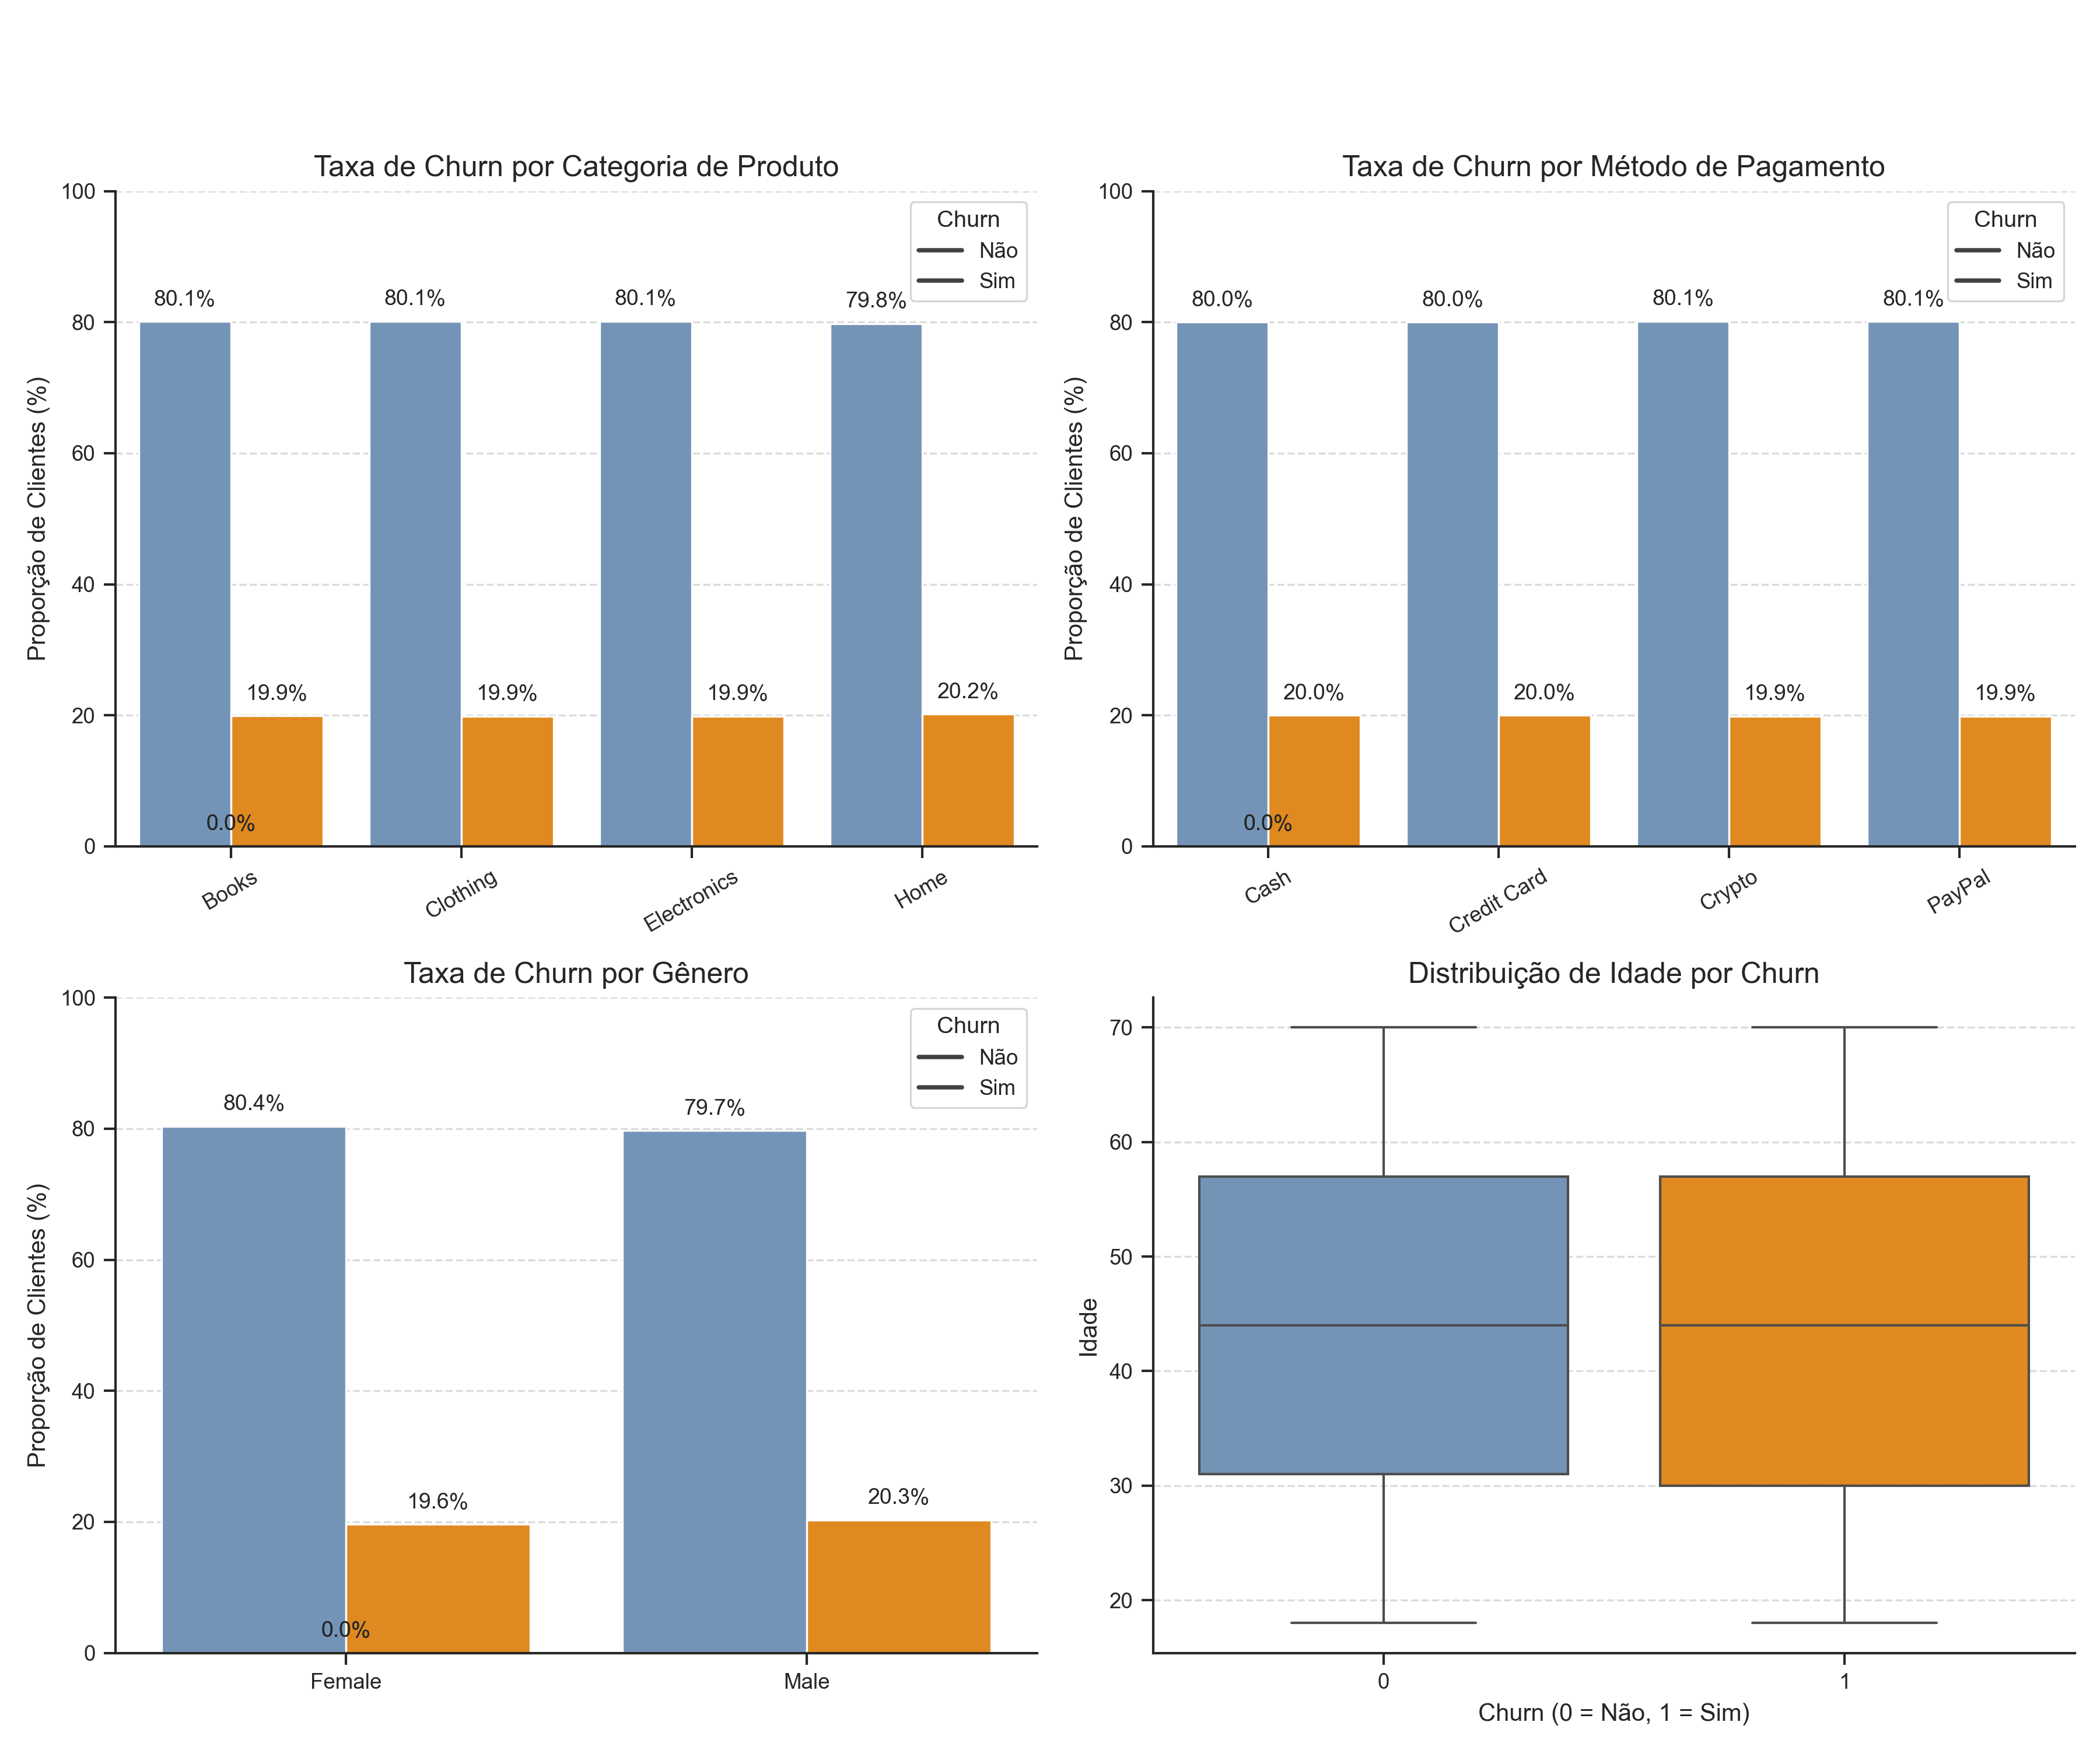
\includegraphics[width=\textwidth]{Imagens/bivariada_churn.png}
	\caption{Análise bivariada das variáveis em relação ao Churn.}
	\label{fig:bivariada_churn}
\end{figure}
\begin{flushleft}
\footnotesize Fonte: Elaborado pelo autor (2025).
\end{flushleft}

A análise visual dos gráficos indica que a proporção de churn em relação ao não-churn é visualmente semelhante em todas as categorias de produto, métodos de pagamento e gêneros. Adicionalmente, a distribuição de idade entre os clientes que são churn e os que não são é praticamente idêntica, o que foi confirmado por uma análise numérica detalhada que mostrou medianas e médias de idade iguais para ambos os grupos.

Esta ausência de um sinal claro em preditores simples e estáticos é um resultado crucial. Constatou-se que as variáveis demográficas, bem como as características de compra, não apresentaram, de forma isolada, uma correlação forte com a decisão de um cliente abandonar a plataforma. Esse achado reforça a escolha da Análise de Sobrevivência como metodologia central, pois sugere que o comportamento de churn é provavelmente impulsionado por fatores mais dinâmicos e temporais, como a frequência das compras e o tempo entre elas.

\subsection{Análise de Sobrevivência}
Nesta seção, são apresentados os resultados obtidos com a aplicação dos modelos de sobrevivência, que visam analisar o tempo até a ocorrência de uma nova compra, utilizando os dados previamente tratados e preparados.

\subsubsection{Análise Exploratória das Variáveis de Sobrevivência}
Antes da modelagem, foi realizada uma análise exploratória para entender como as variáveis de sobrevivência recém-criadas, \texttt{evento} e \texttt{duracao}, se relacionam com as demais características dos clientes.

A Figura \ref{fig:analise_vs_evento} investiga se alguma característica está associada a uma compra ser a última observada para um cliente (evento = 0).

\begin{figure}[h!]
	\centering
	% Substitua 'analise_vs_evento.png' pelo nome do seu arquivo de imagem
	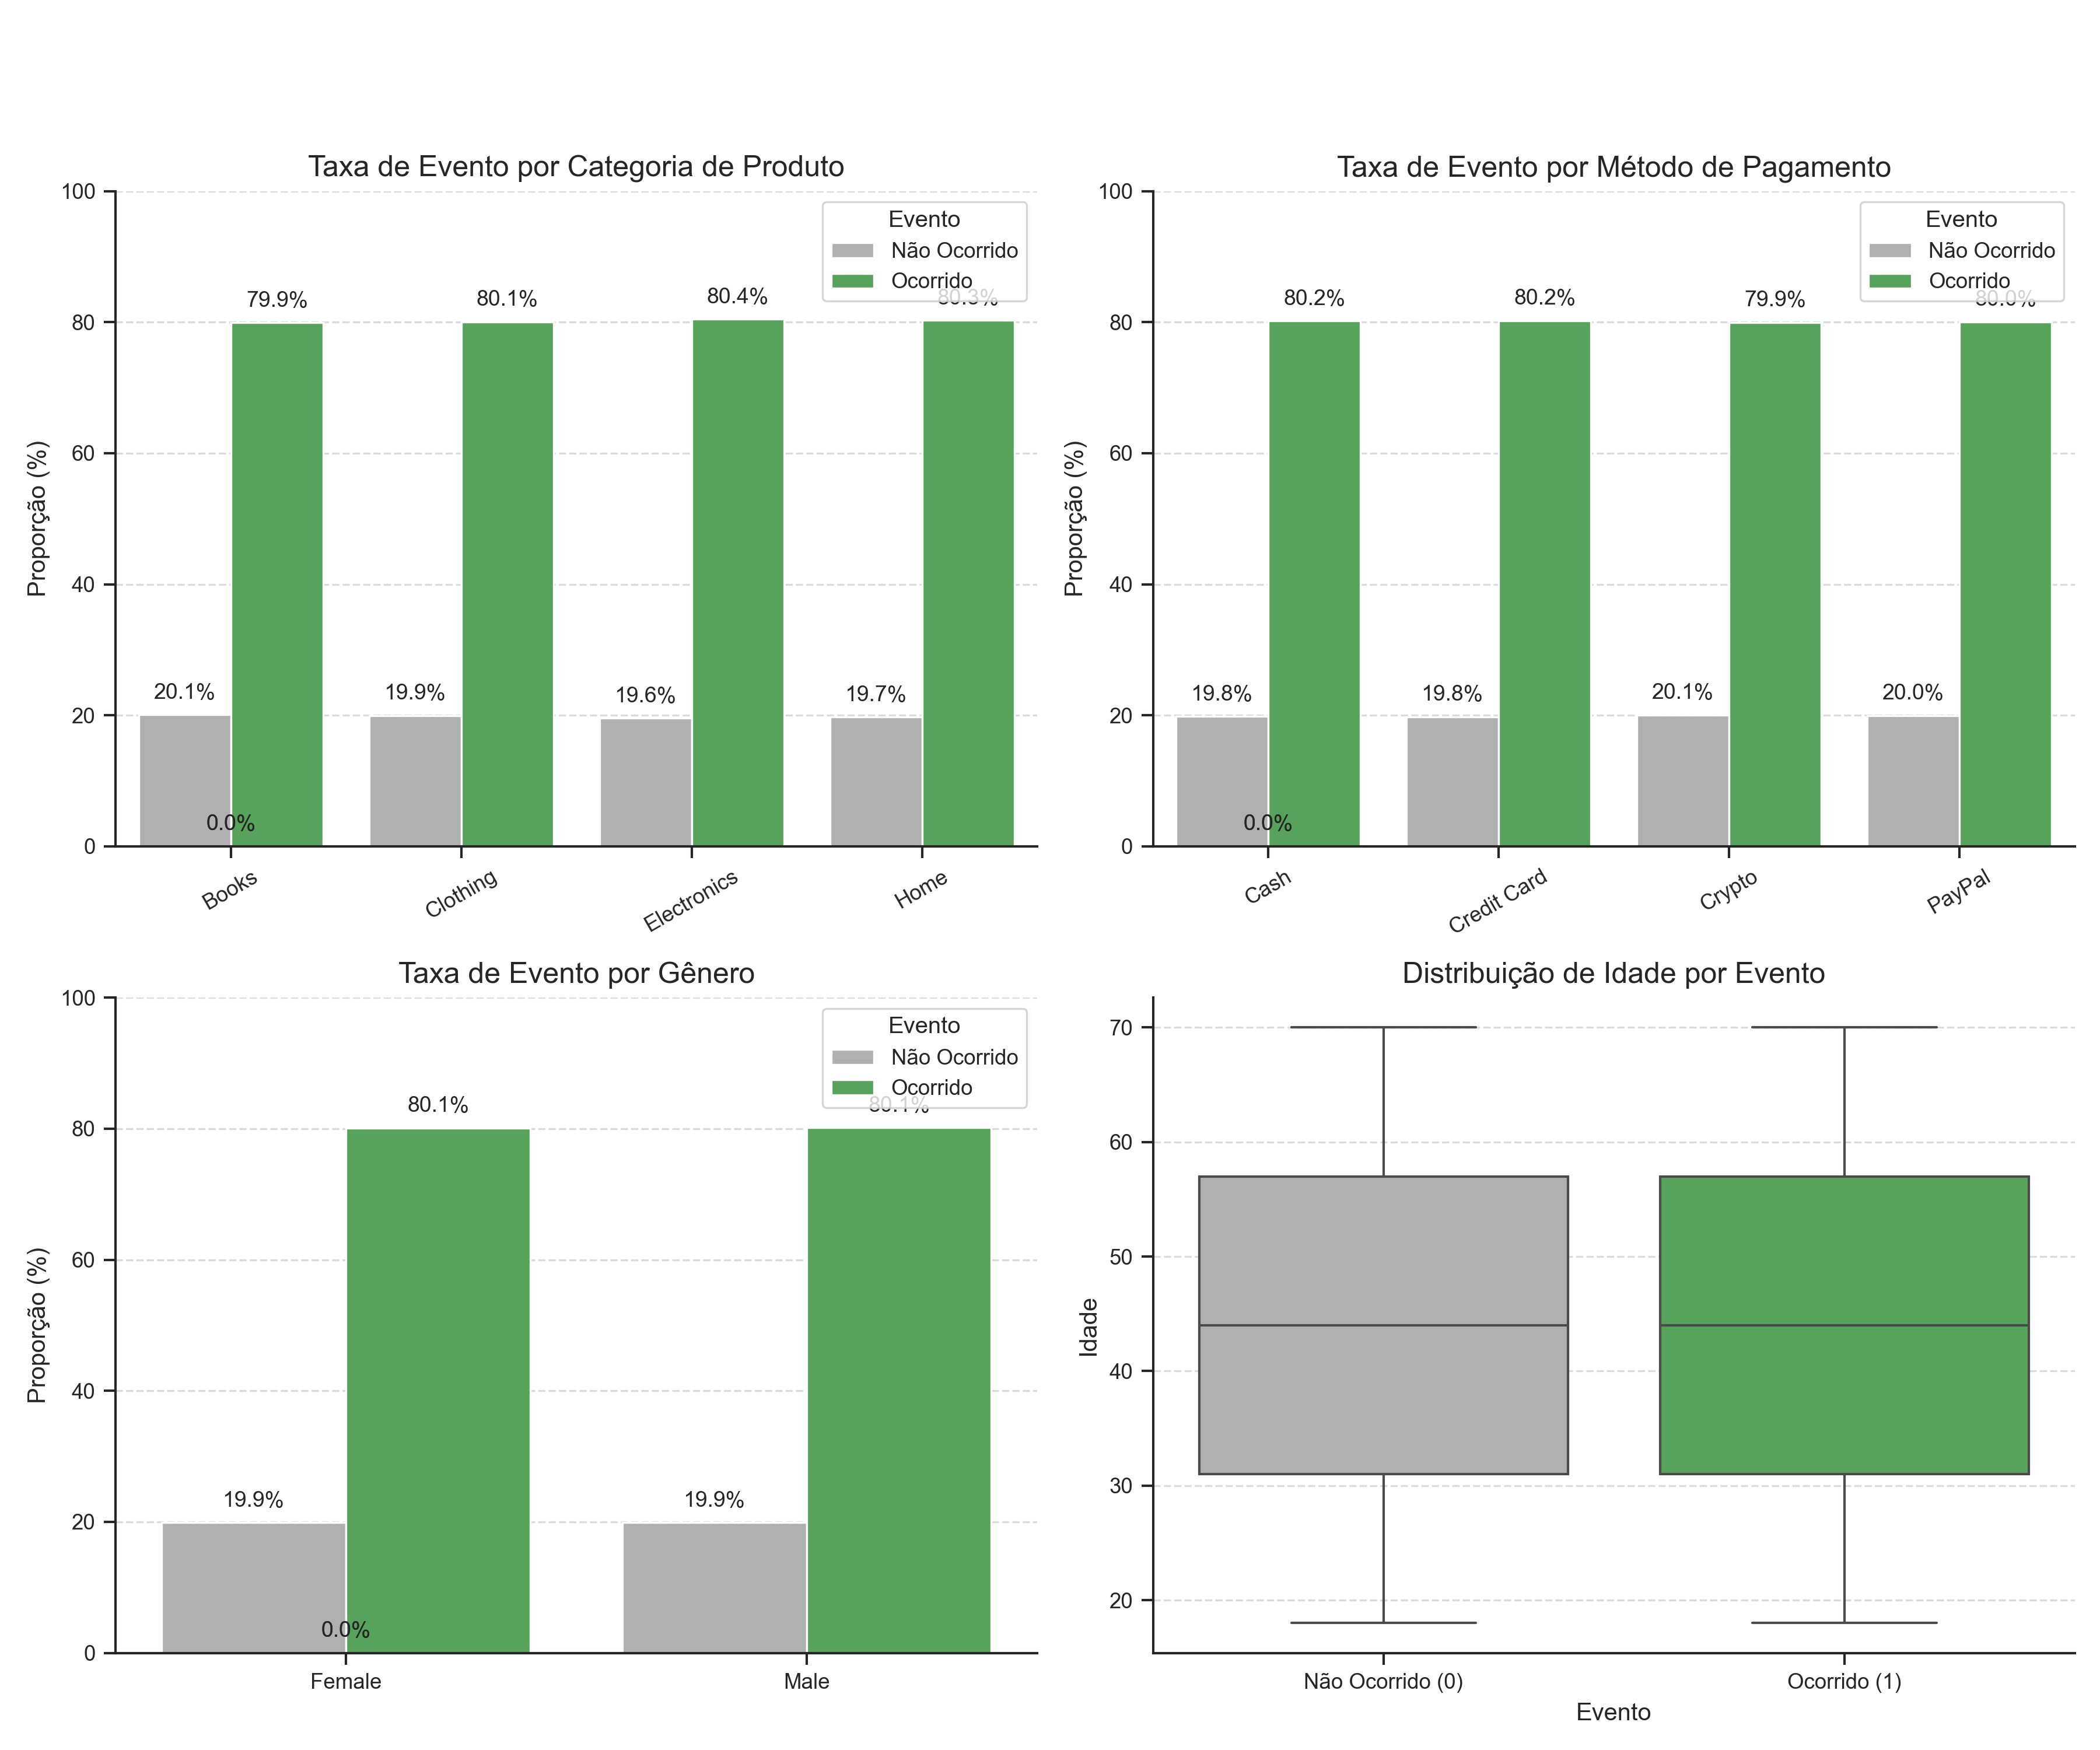
\includegraphics[width=\textwidth]{Imagens/analise_vs_evento.png}
	\caption{Análise Bivariada de covariáveis vs. a variável \texttt{evento}.}
	\label{fig:analise_vs_evento}
\end{figure}
\begin{flushleft}
\footnotesize Fonte: Elaborado pelo autor (2025).
\end{flushleft}

A análise da Figura \ref{fig:analise_vs_evento} mostra que a proporção de evento=0 (compra final observada) para evento=1 (recompra) é visualmente a mesma em todas as categorias de produto, métodos de pagamento e gêneros. Adicionalmente, a distribuição de idade, representada pelos boxplots, é idêntica para ambos os desfechos. A conclusão é que nenhuma dessas variáveis estáticas parece influenciar a probabilidade de uma compra ser a última registrada de um cliente.

A seguir, a Figura \ref{fig:analise_vs_duracao} analisa se o tempo até a próxima compra (\texttt{duracao}) varia entre diferentes grupos de clientes.

\begin{figure}[h!]
	\centering
	% Substitua 'analise_vs_duracao.png' pelo nome do seu arquivo de imagem
	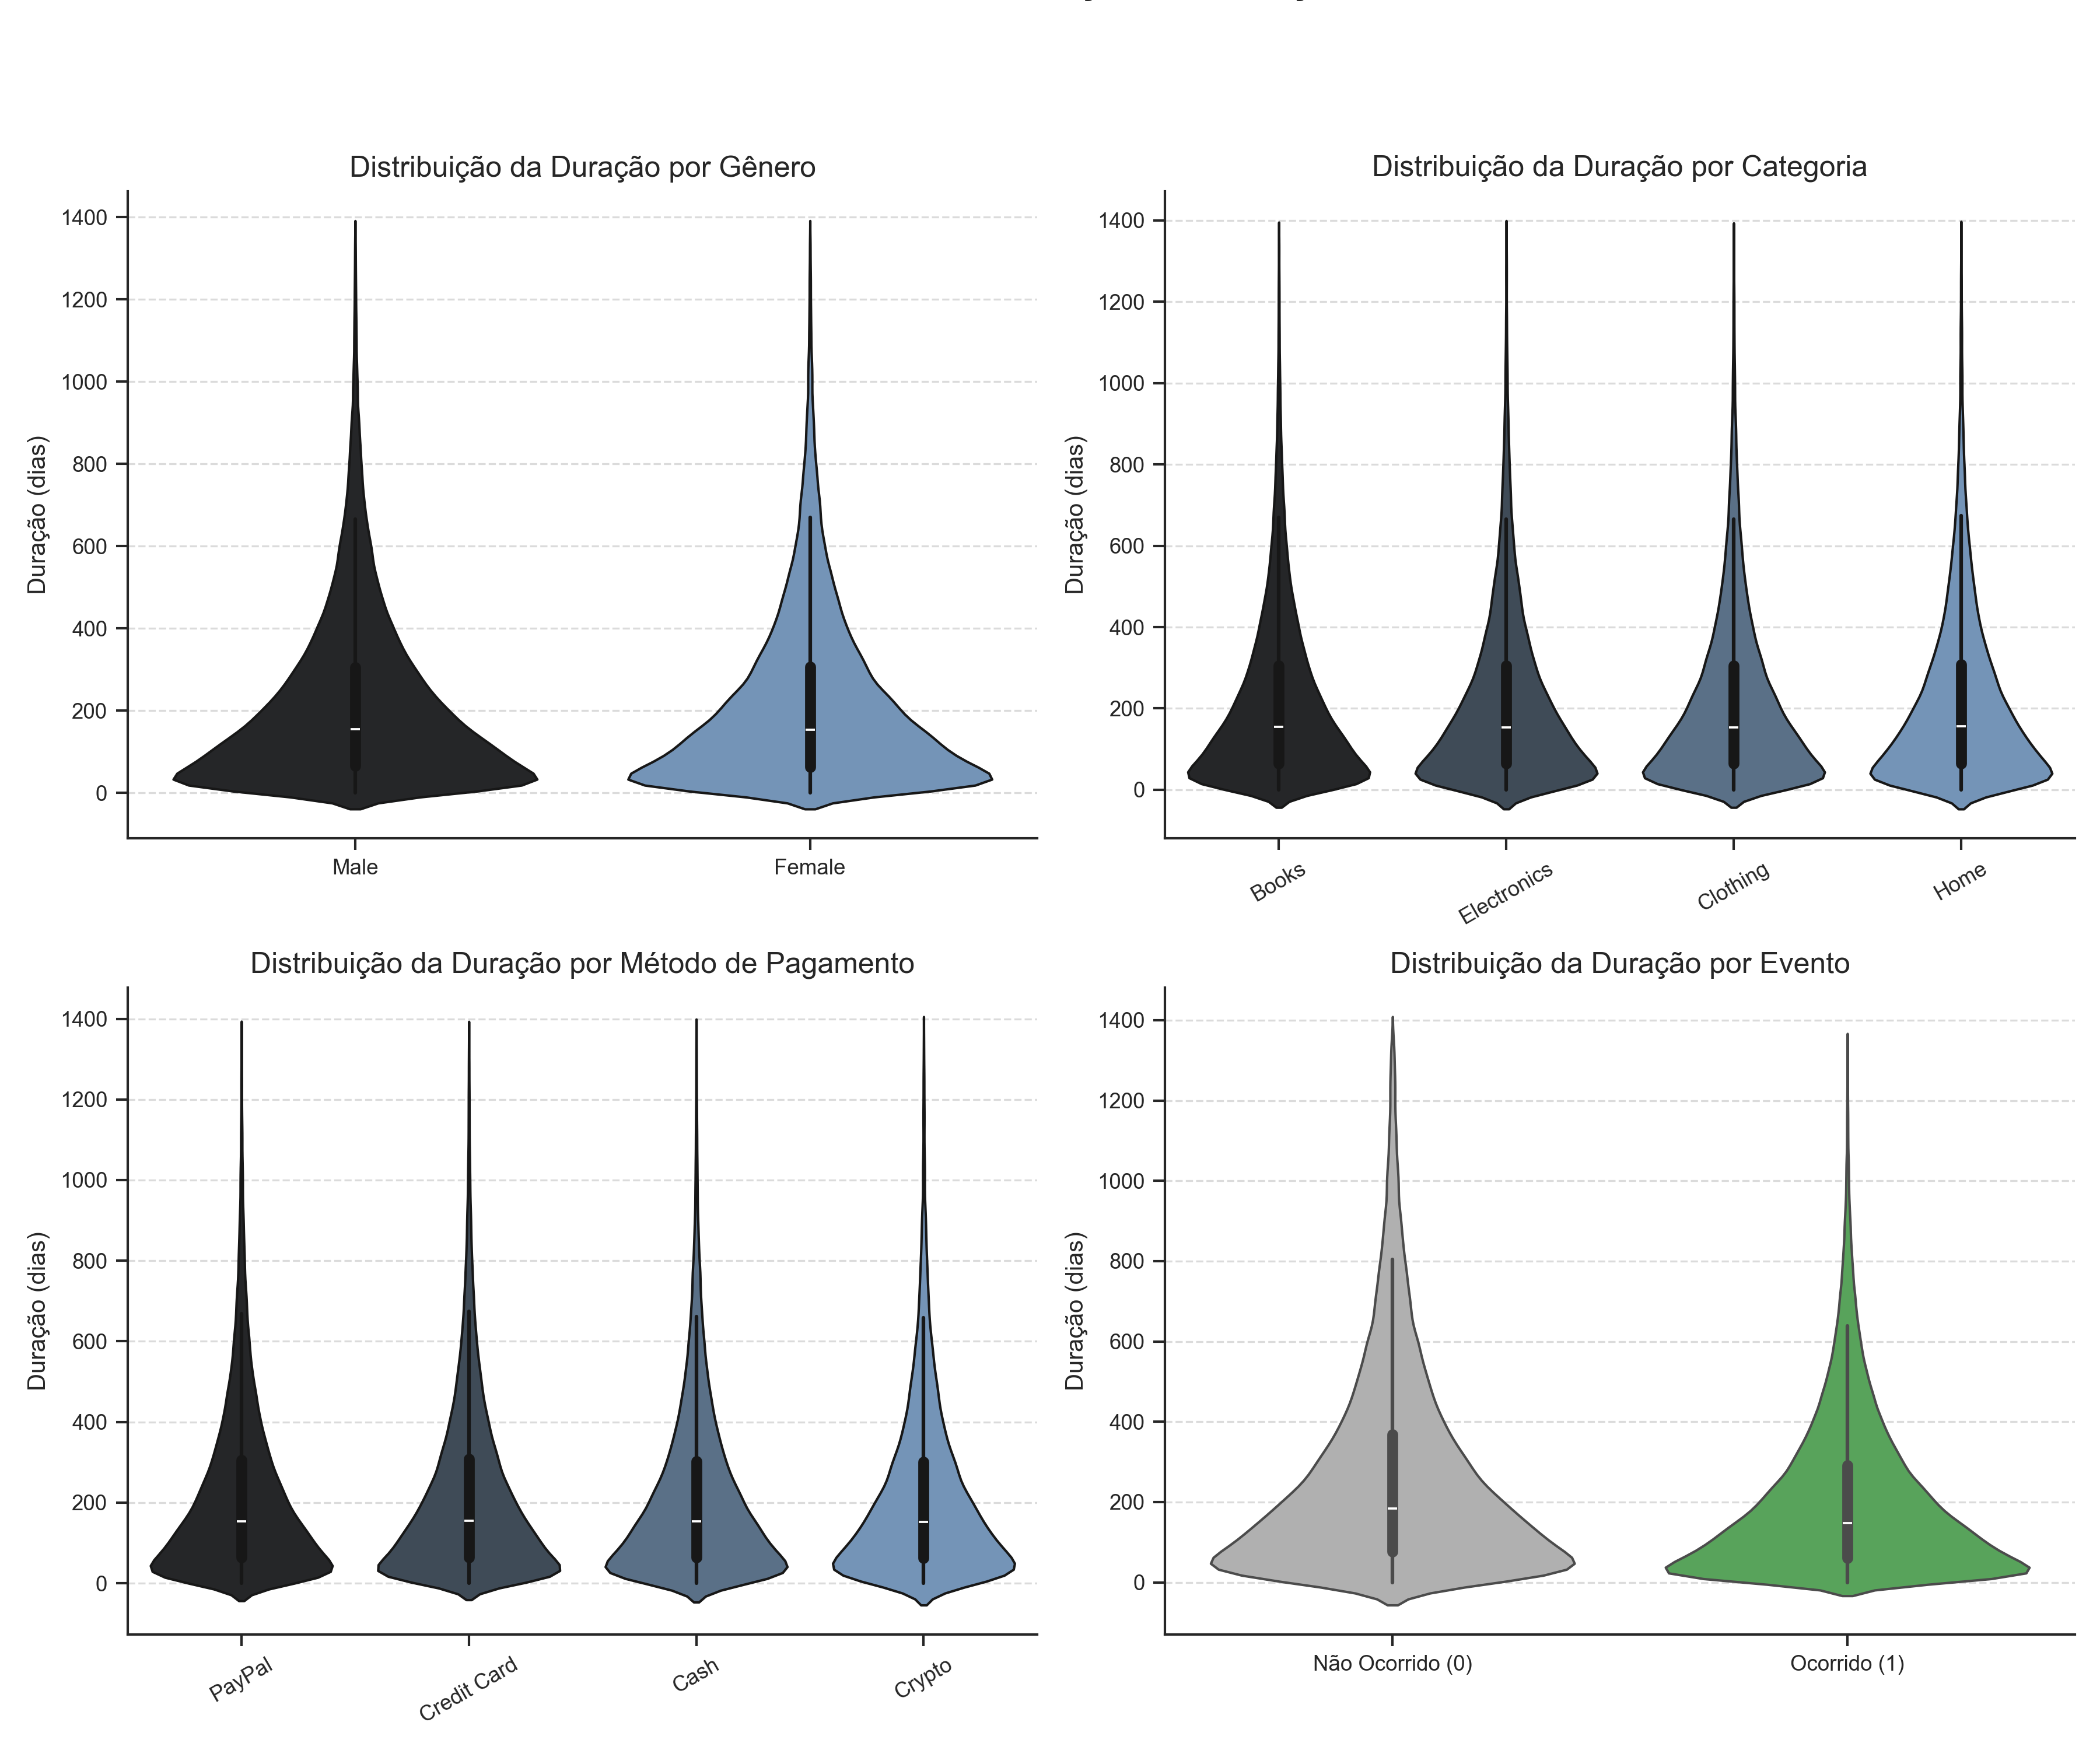
\includegraphics[width=\textwidth]{Imagens/analise_vs_duracao.png}
	\caption{Análise Bivariada de covariáveis vs. a variável \texttt{duracao}.}
	\label{fig:analise_vs_duracao}
\end{figure}
\begin{flushleft}
\footnotesize Fonte: Elaborado pelo autor (2025).
\end{flushleft}

A partir dos gráficos de violino, observa-se que a distribuição da duração é praticamente idêntica entre os gêneros, as categorias de produto e os métodos de pagamento. Este é um achado importante, pois sugere que o ciclo de recompra não é influenciado por essas características. Em contrapartida, a distribuição da duração por evento é drasticamente diferente: as durações para recompras (evento=1) são, em média, mais curtas, enquanto as durações para dados censurados (evento=0) são naturalmente mais longas, o que valida a engenharia de atributos realizada.


\subsubsection{Análise Não-Paramétrica: Estimador de Kaplan-Meier}
A análise inicial foi a estimação da função de sobrevivência geral para toda a base de clientes utilizando o estimador de Kaplan-Meier. A curva resultante, apresentada na Figura \ref{fig:km_geral}, mostra a probabilidade de um cliente "sobreviver" (ou seja, não realizar uma nova compra) ao longo do tempo.

\begin{figure}[h!]
	\centering
	% Substitua 'kaplan_meier_geral.png' pelo nome do seu arquivo de imagem
	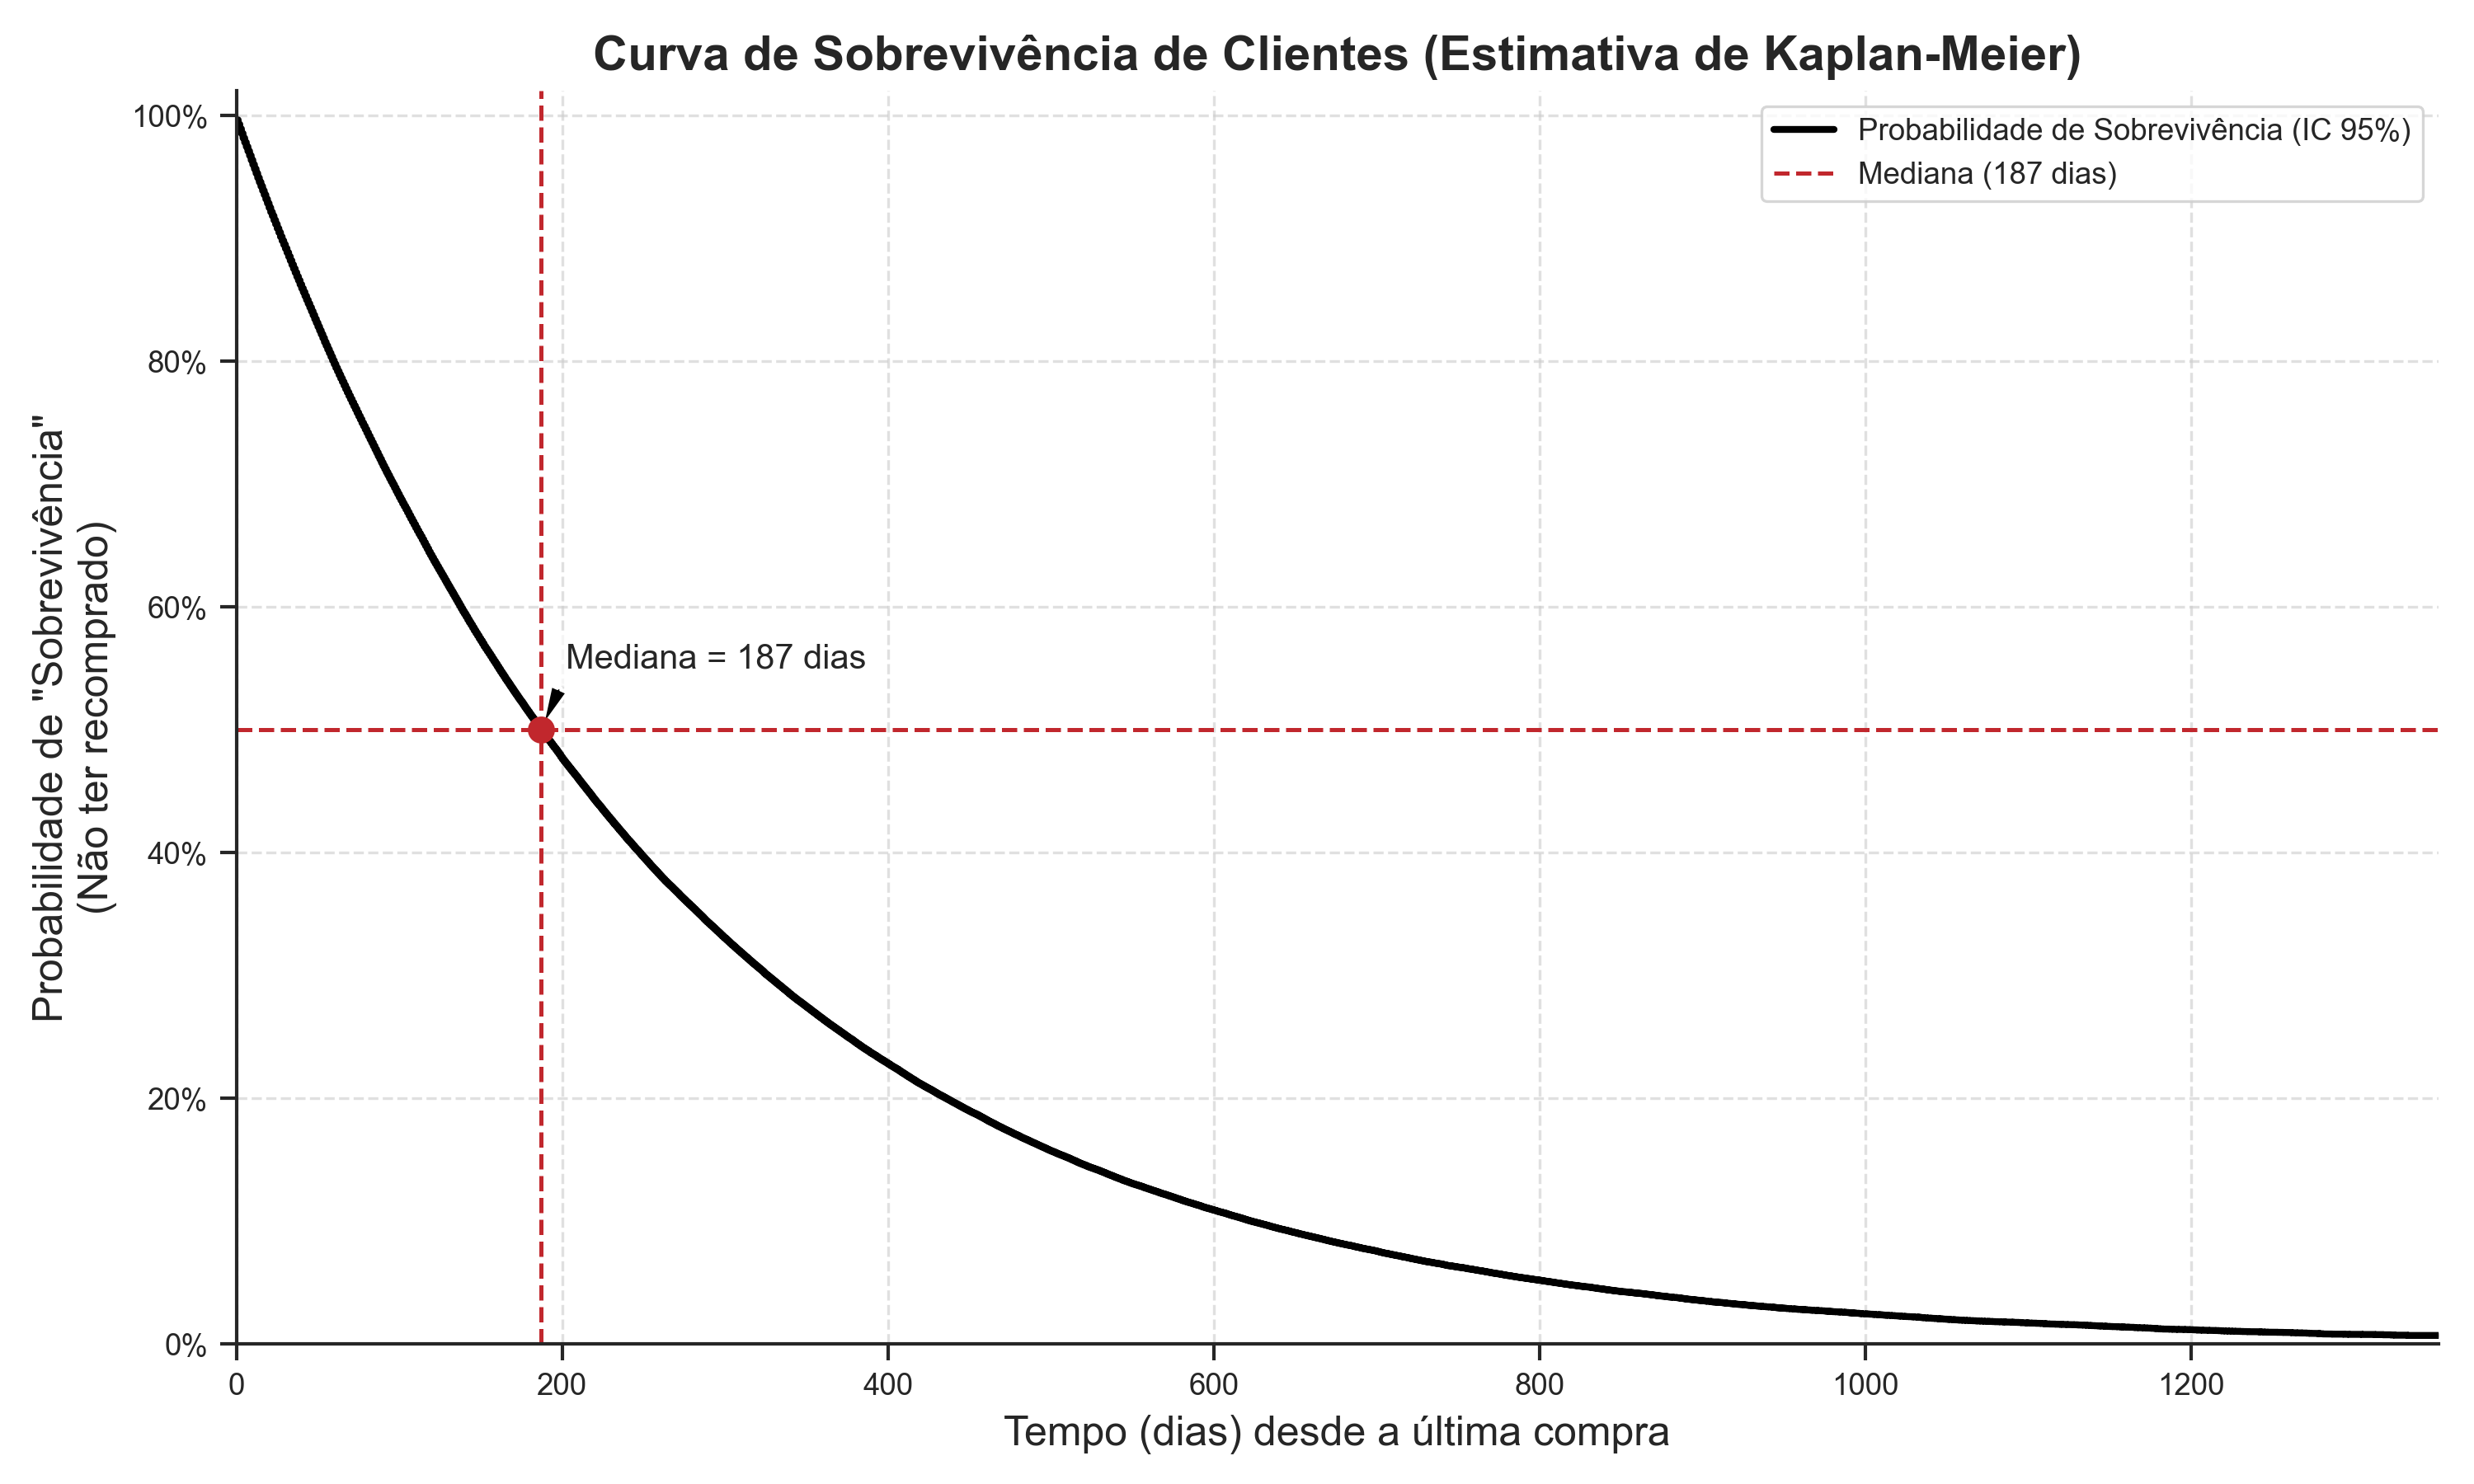
\includegraphics[width=0.8\textwidth]{Imagens/kaplan_meier_geral.png}
	\caption{Curva de Sobrevivência de Clientes (Estimador de Kaplan-Meier).}
	\label{fig:km_geral}
\end{figure}
\begin{flushleft}
\footnotesize Fonte: Elaborado pelo autor (2025).
\end{flushleft}


A curva de Kaplan-Meier revela um declínio acentuado nos primeiros meses, indicando que a probabilidade de um cliente não comprar novamente diminui rapidamente. O principal resultado desta análise é a \textbf{mediana do tempo de sobrevivência}, que foi de \textbf{187 dias}. Isso significa que 50\% dos clientes que realizam uma nova compra o fazem em até 187 dias após a compra anterior.

Para investigar se diferentes grupos de clientes possuíam comportamentos de recompra distintos, as curvas de sobrevivência foram comparadas utilizando o teste Log-Rank. Foram analisados os grupos por Gênero, Volume de Compra e Categoria de Produto. Em todas as comparações, as curvas de sobrevivência dos diferentes grupos se mostraram praticamente idênticas e sobrepostas.

Os resultados dos testes Log-Rank confirmaram a observação visual:
\begin{itemize}
    \item \textbf{Gênero:} O teste não mostrou diferença estatisticamente significativa entre os gêneros masculino e feminino (p-valor = 0.85).
    \item \textbf{Volume de Compra:} Não houve diferença significativa entre os grupos de volume de compra baixo, médio e alto (p-valor = 0.18).
    \item \textbf{Categoria de Produto:} O comportamento de recompra também se mostrou idêntico entre as quatro categorias de produto (p-valor = 0.51).
\end{itemize}

A análise não-paramétrica concluiu, portanto, que o comportamento de recompra dos clientes neste dataset é notavelmente homogêneo. Fatores como gênero, valor gasto ou categoria do produto não se mostraram, isoladamente, preditores do tempo que um cliente levará para fazer uma nova compra.

\subsubsection{Análise Semi-Paramétrica: Modelo de Riscos Proporcionais de Cox}
Para avaliar o efeito simultâneo de múltiplas variáveis sobre a probabilidade de recompra, foi ajustado um modelo de Riscos Proporcionais de Cox. O desempenho geral do modelo foi avaliado pelo \textbf{Índice de Concordância (C-index)}, cujo valor foi de \textbf{0.50}. Um C-index de 0.5 indica que o modelo não possui poder preditivo, sendo equivalente a uma decisão aleatória para prever qual de dois clientes irá recomprar primeiro. Este resultado corrobora os achados da análise não-paramétrica, indicando que as variáveis utilizadas não são bons preditores do tempo de recompra.

A análise dos coeficientes individuais do modelo, detalhada na Tabela \ref{tab:cox_summary}, reforça essa conclusão.

% Tabela Resumo do Modelo de Cox (simplificada para as colunas mais importantes)
\begin{table}[h!]
\centering
\caption{Resumo do resultado do Modelo de Cox.}
\label{tab:cox_summary}
\begin{tabular}{lrrrrr}
\hline
\textbf{Covariável} & \textbf{coef} & \textbf{exp(coef)} & \textbf{se(coef)} & \textbf{p} \\
\hline
Age & 0.00 & 1.00 & 0.00 & 0.94	 \\
Total Purchase Amount & -0.00 & 1.00 & 0.00 & > 0.42 \\
Quantity & -0.00 & 1.00 & 0.00 & > 0.14 \\
\textbf{Returns} & \textbf{0.01} & \textbf{1.01} & \textbf{0.00} & \textbf{0.01} \\
Gender\_Male & -0.00 & 1.00 & 0.00 & 0.85 \\
Product\_Category\_Clothing & 0.00 & 1.00 & 0.01 & 0.78 \\
Product\_Category\_Electronics & 0.01 & 1.01 & 0.01 & 0.24 \\
Product\_Category\_Home & -0.00 & 1.00 & 0.01 & 0.65 \\
Payment\_Method\_Credit\_Card & -0.01 & 0.99 & 0.01 & 0.08 \\
Payment\_Method\_Crypto & 0.00 & 1.00 & 0.01 & 0.65 \\
Payment\_Method\_PayPal & -0.01 & 0.99 & 0.01 & 0.15 \\
\hline
\end{tabular}
\end{table}
\begin{flushleft}
\footnotesize Fonte: Elaborado pelo autor (2025).
\end{flushleft}

Com exceção da variável \texttt{Returns}, todas as outras covariáveis apresentaram p-valores maiores que 0.05, não sendo estatisticamente significativas. A variável \texttt{Returns} foi significativa (p=0.01), com uma razão de risco (\textit{hazard ratio}, ou \texttt{exp(coef)}) de 1.01. Isso indica que clientes que devolvem uma compra têm um "risco" de recomprar 1\% maior em qualquer ponto no tempo, ou seja, tendem a realizar a próxima compra de forma marginalmente mais rápida. No entanto, o efeito, apesar de estatisticamente significante, é muito pequeno e não altera a conclusão geral sobre a falta de fortes preditores no modelo.

